%!TEX root = ../../../adrien_gomar_phd.tex

Consider for simplicity a turbomachinery stage composed of two rotors,
as for instance a CROR configuration.
A wake is shed behind
the upstream and the downstream rotor. 
It is stationary in the frame of reference attached to the upstream wheel.
\begin{figure}[htp]
    \centering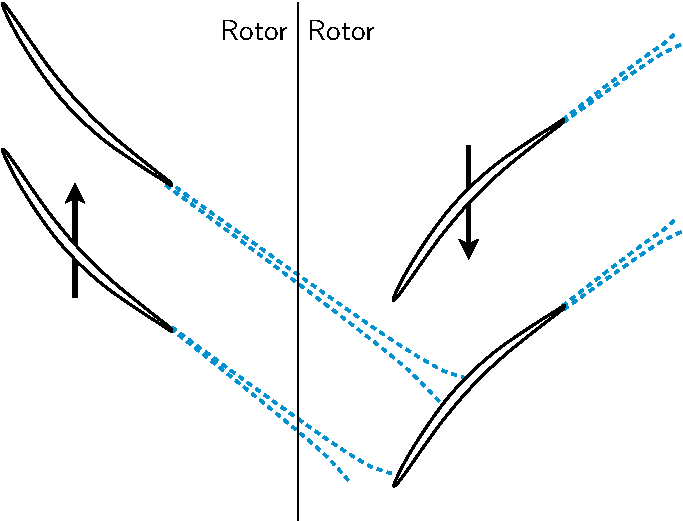
\includegraphics[width=.35\textwidth]{cror_wakes.pdf}
  \caption{Characteristic wakes in a CROR configuration.}
  \label{fig:rotor-stator}
\end{figure}
However, when it crosses the rotor-rotor interface,
the wake becomes unsteady in the frame of reference of the second wheel. 
Thus, an upstream steady spatial distortion becomes unsteady in
the downstream row.

\citet{Lakshminarayana1980} showed that the wake
behind turbomachinery blades follows a similarity law for the velocity. 
It can be empirically approximated by a Gaussian function:
\begin{equation}
    u_l (t) = u_m \left[1 - 
        \Delta u \cdot e^{
          -0.693 \left(\frac{2 c t}{L_x L} \right) ^ 2}\right],
    \label{eq:similarity}
\end{equation}
where $u_m$ denotes the free-stream velocity, $\Delta u$ the axial wake velocity deficit,
$\theta$ the azimuthal coordinate and $L$ the wake width,
defined as the full width at half maximum.

Therefore, in the downstream frame of reference, wakes coming 
from the upstream wheel can be represented, 
to a first approximation, as the periodic 
advection of a Gaussian function from the inter-wheel interface.

To study the convergence properties of such a function,
we consider again the linear advection problem defined in Sec.~\ref{sec:linear}, 
with $u_l$ now taken equal to a Gaussian function.
The full width at half maximum $L$ of the wake is set to 10\% of the domain size, 
$u_m$ is set to $c$ and $\Delta u$ to 10\% of $u_m$.

\begin{figure}[htp]
  \centering
  \subfigure[$N=1$]{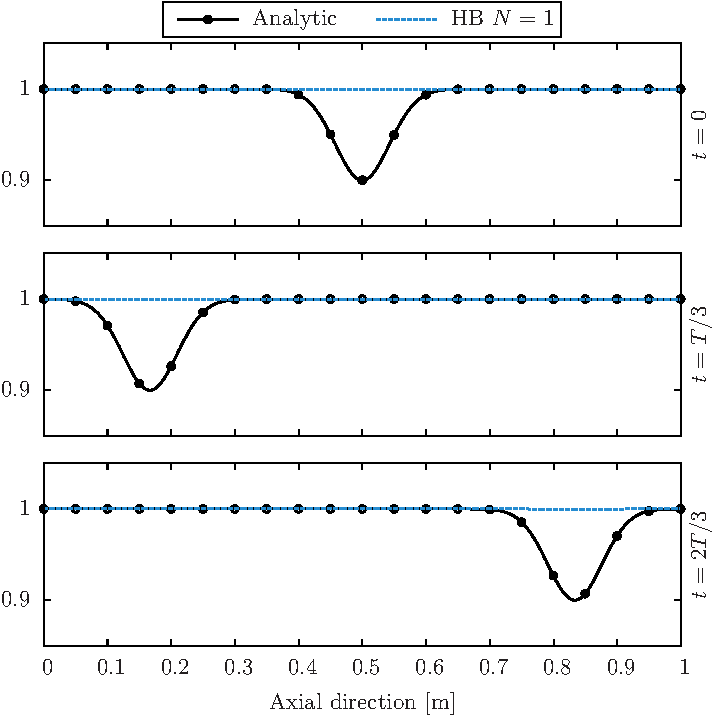
\includegraphics[width=.35\textwidth]{convection_wake_N1.pdf}}
  \subfigure[$N=2$]{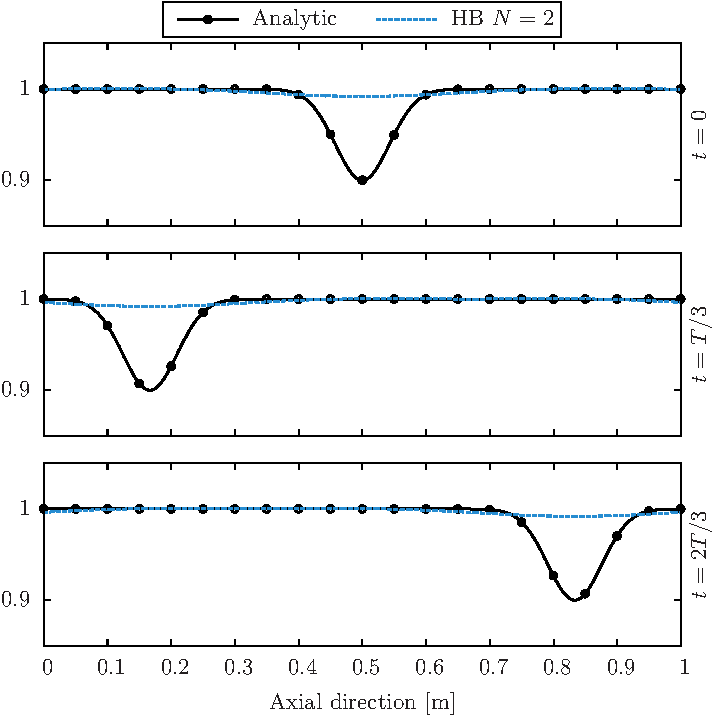
\includegraphics[width=.35\textwidth]{convection_wake_N2.pdf}}
  \subfigure[$N=3$]{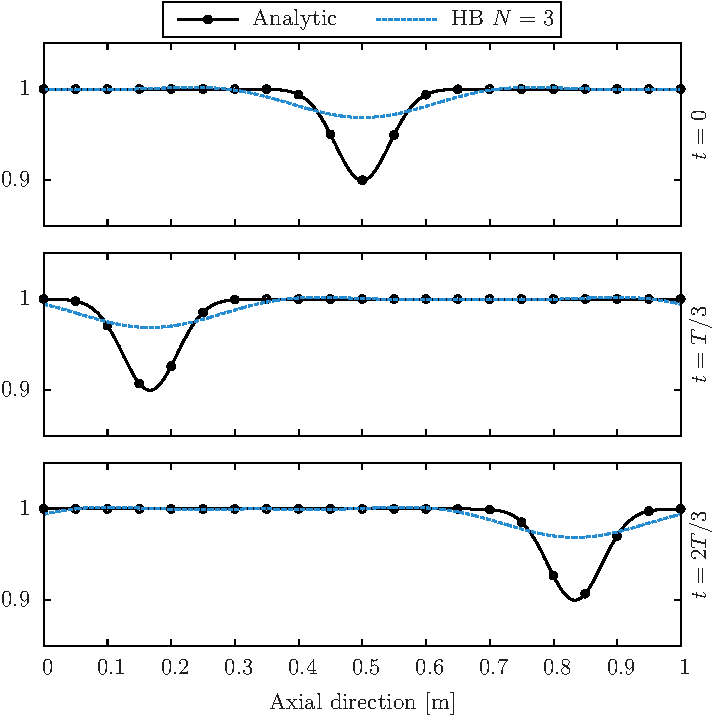
\includegraphics[width=.35\textwidth]{convection_wake_N3.pdf}}
  \subfigure[$N=4$]{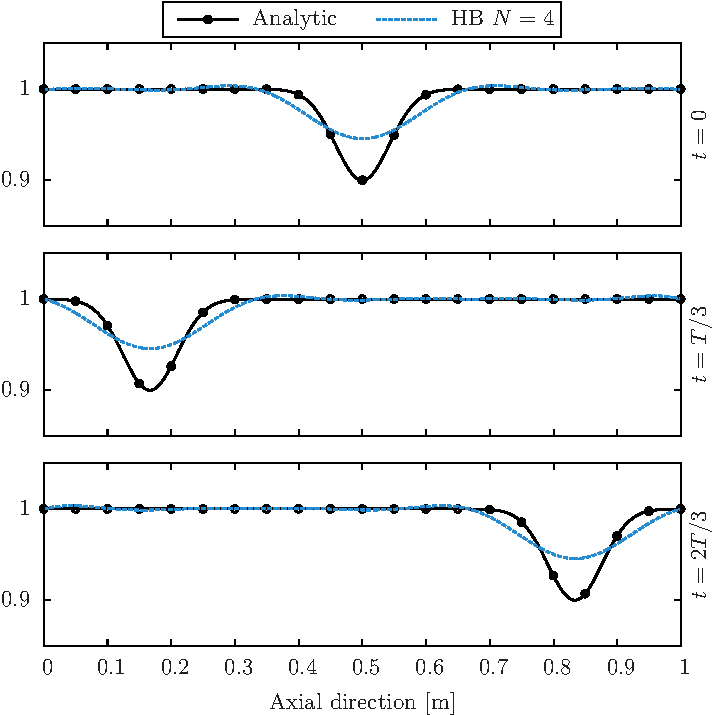
\includegraphics[width=.35\textwidth]{convection_wake_N4.pdf}}
  \subfigure[$N=5$]{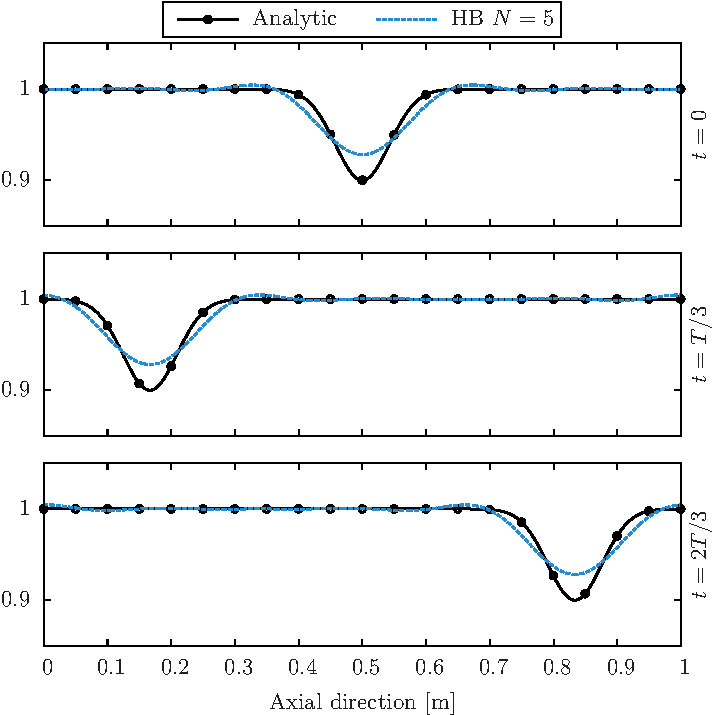
\includegraphics[width=.35\textwidth]{convection_wake_N5.pdf}}
  \subfigure[$N=6$]{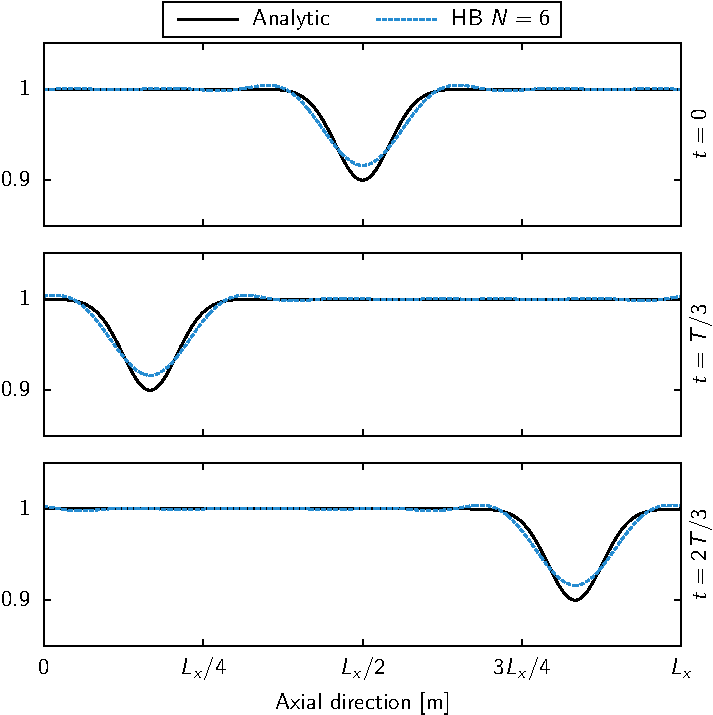
\includegraphics[width=.35\textwidth]{convection_wake_N6.pdf}}
  \caption{Linear advection of a Gaussian function representing a turbomachinery wake: 
  numerical solutions at different time instances for different numbers of harmonics.}
  \label{fig:inj_wake_results}
\end{figure}
Figure~\ref{fig:inj_wake_results} depicts the HB
computations for one to six harmonics. The numerical solution convergences
to the exact Gaussian function starting from $N=6$ harmonics.
When the number of harmonics is
too small, the width and the depth of the wake are badly approximated
by the method, and the solution exhibits some spurious oscillations. 

\begin{figure}[htp]
  \centering
  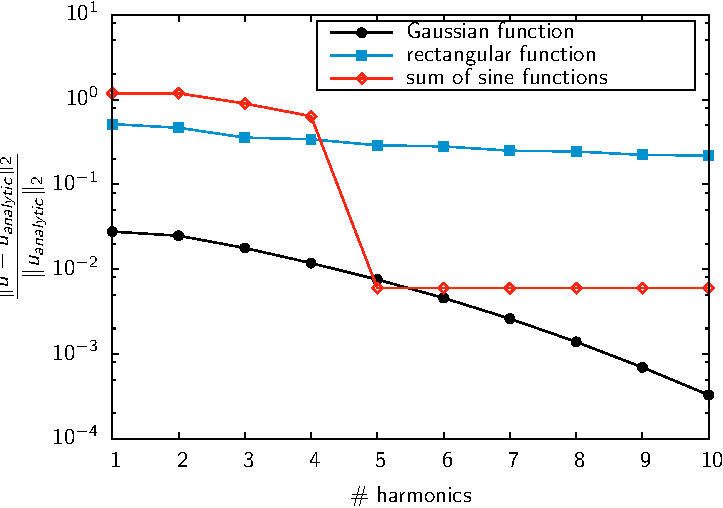
\includegraphics[width=.5\textwidth]{convection_wake_error.pdf}
  \caption{Linear advection of a Gaussian function representing a 
  turbomachinery wake: convergence of the HB method error.}
  \label{fig:conv_wake}
\end{figure}
Figure~\ref{fig:conv_wake} shows the quantitative convergence of 
the $\mathcal{L}_2$ error. The
convergence curves for the two functions studied in the previous sections
are also reported for comparison.
The error follows now a nearly exponential convergence.
\begin{figure}[htp]
  \centering
  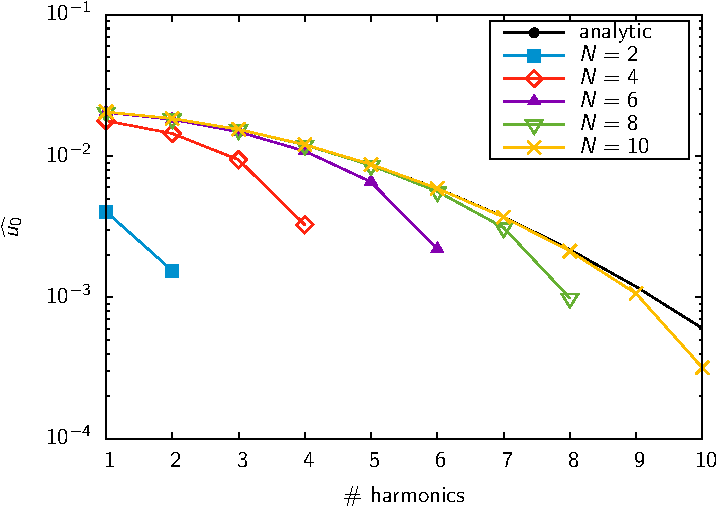
\includegraphics[width=.5\textwidth]{convection_wake_dft.pdf}
  \caption{Linear advection of a Gaussian function representing a turbomachinery wake: 
  discrete Fourier transform.}
  \label{fig:dft_wake}
\end{figure}
The discrete Fourier transform of the results is
depicted against the analytical result in Figure~\ref{fig:dft_wake}.
The $N=2$ and $N=4$ computations badly capture the amplitudes of the
resolved harmonics.
Starting from $N=6$, some of the lower 
frequencies are correctly captured, whereas high frequencies are
always under-estimated.
This improves when further harmonics are added to the computation.

For a better understanding of the HB convergence behavior, 
we consider the spectral content of the Gaussian wake model. 
Precisely, the Fourier transform $\widehat{g}$ of a Gaussian function $g$
defined as
\begin{equation}
    g(x) = A e^{-\alpha x^2},
    \label{eq:simple_gaussian_function}
\end{equation}
where $A$ and $\alpha$ are constants, is
\begin{equation}
    \widehat{g}(f) = A^\prime e^{-\alpha^\prime f^2},
    \label{eq:fourier_transform_gaussian}
\end{equation}
where
\begin{equation}
  \begin{cases}
    A^\prime=A \sqrt{\frac{\pi}{\alpha}},\\
    \alpha^\prime = \frac{\pi^2}{\alpha}.
  \end{cases}
\end{equation}
For the similarity law of Lakshminarayana and Davino, 
$\alpha$ and $\alpha^\prime$ can be identified as
\begin{equation}
    \alpha =  0.693 \left( \frac{2}{L} \right)^2, \quad
    \alpha^\prime =  \frac{1}{0.693} \left( \frac{\pi L}{2} \right)^2.
    \label{eq:gaussian_params_laksh}
\end{equation}
The exponential factor of the wake law~$\alpha$ is inversely
proportional to its Fourier counter-part~$\alpha'$, meaning that their
width will vary in opposite way: the thinner the wake, the wider its
spectrum and \emph{vice-versa}.

The convergence rate is inherently linked to
the spectrum of the considered unsteady signal.
As for the present case we know the analytical wake spectrum,
we define the theoretical truncation error as the ratio of
the energy contained in the unresolved part 
of the spectrum to the overall energy content of the full spectrum
\begin{equation}
    \varepsilon_{th}(f) = \sqrt{\frac{
        \int_f^\infty | \widehat{g}(\zeta)|^2 \diff \zeta
      }{
        \int_0^\infty | \widehat{g}(\zeta)|^2 \diff \zeta
      }}.
    \label{eq:def_truncation_error}
\end{equation}
Introducing the error function defined as
\begin{equation}
    \erf(x) = \frac{2}{\sqrt{\pi}} \int_0^x e^{-t^2} \diff t,
\end{equation}
and the complementary error function defined as
\begin{equation}
    \erfc(x) = 1 - \erf(x),
\end{equation}
then
\begin{align}
    \int_0^\infty | \widehat{g}(\zeta)|^2 \diff \zeta 
    &= \frac{1}{2} \int_{- \infty}^\infty | \widehat{g}(\zeta)|^2 \diff \zeta \\
    &= \frac{A^{\prime 2}}{2} \sqrt{\frac{\pi}{2 \alpha^\prime}},
\end{align}
and
\begin{equation}
    \int_f^\infty | \widehat{g}(\zeta)|^2 \diff \zeta = 
      \frac{A^{\prime 2}}{2} \sqrt{\frac{\pi}{2 \alpha^\prime}} \erfc (\sqrt{2 \alpha^\prime} f).
\end{equation}
The theoretical truncation error can then be written as
\begin{equation}
    \varepsilon_{th}(f, L) = \sqrt{\erfc (\sqrt{2 \alpha^\prime(L) } f)}.
    \label{eq:analytical_conv}
\end{equation}
One can notice from Eq.~\eqref{eq:analytical_conv} that the 
truncation error does not depend on the wake deficit $\Delta u$ 
but only on the wake width $L$.

\begin{figure}[htp]
    \centering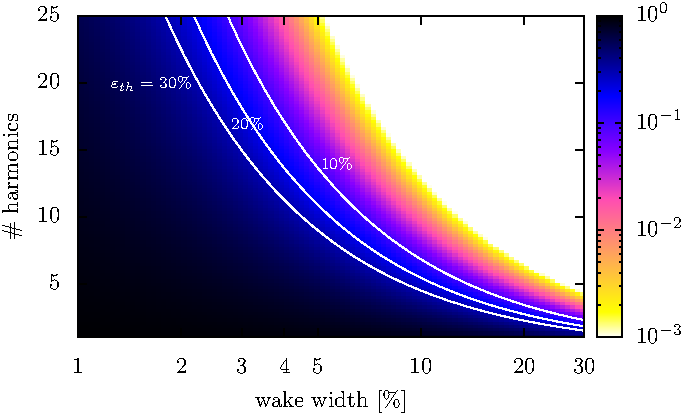
\includegraphics[width=.5\textwidth]{ANALYTICAL_ERROR_PPT.pdf}
  \caption{Theoretical truncation error of the Lakshminarayana and Davino wake law.}
  \label{fig:analytic_error_paper}
\end{figure}
Eq.~\eqref{eq:analytical_conv} is depicted in
Figure~\ref{fig:analytic_error_paper} for varying
number of harmonics and wake widths.
It can be seen that the wider the spectrum,
the higher the number of harmonics needed to
reach a certain level of error. 
Moreover, for a thin wake width (\emph{e.g.} 2\% of the pitch)
the number of harmonics required to capture it with a truncation 
error of 10\% is up to 25~harmonics.
In the limit of $L \to 0$, the wake becomes a Dirac function
which represents the worst possible case, as the rectangular
function was.
In the preceding example, the Gaussian function had a width
of 10\% which, according to Eq.~\eqref{eq:analytical_conv},
is captured by using $N=7$ harmonics for a target 10\% error.

This section provided analytical results of the
convergence of Fourier-based time methods 
in the case of wake passing. To confirm these results,
a turbomachinery like model problem
is set up and solved using the Euler equations in
the following section.



